\documentclass[runningheads,a4paper]{llncs}

\usepackage{amssymb}
\setcounter{tocdepth}{3}
\usepackage{graphicx}

\usepackage{url}
\newcommand{\keywords}[1]{\par\addvspace\baselineskip
\noindent\keywordname\enspace\ignorespaces#1}

\begin{document}

\mainmatter  % start of an individual contribution

% first the title is needed
\title{Cloud Computing and Big Data\\Coursework Report:\\
Fault Tolerant Cloud Application for Mandelbrot Set}

\titlerunning{Fault Tolerant Cloud Application for Mandelbrot Set}

\author{Jonah Lyu}

\authorrunning{Fault Tolerant Cloud Application for Mandelbrot Set}

\institute{University of Bristol, Bristol, United Kingdom\\}

\toctitle{Lecture Notes in Computer Science}
\tocauthor{Authors' Instructions}
\maketitle


\begin{abstract}
This report is for the coursework of the unit Cloud Computing and Big Data. It introduces the implementation of a cloud application which computes Mandelbrot Set in the embarrassingly parallelisable style, including the use of Zookeeper to build a robust network among clusters of AWS EC2 nodes. Then it will analyse the cost of computing across various settings. Finally, it will discuss the fault-tolerant feature and evaluates the scalability of servers with multiple client connections at the same time.

\keywords{Could Computing, Fault Tolerant, Zookeeper, Iaas, Mandelbrot Set,}

\end{abstract}

\section{Introduction}

The coursework requires to implement a fault-tolerant cloud application which computes an embarrassingly parallelisable task. With this requirement, I first did some researches on the concepts of the embarrassingly parallel task. I finally decided to pick the task to compute the Mandelbrot Set. The first step to implement the cloud application is to build a master and worker network which allows a master to distribute a task to a worker. 

Based on this basic task assignment mechanism, I developed an election system which can pick a master from all master candidates to ensure that there is always existing a master in the cluster. The final step is to implement a client that is able to create tasks repeatedly. The task of this application will always include a slice of the Mandelbrot Set figure. Each worker's job is simply waiting for a task to be assigned and computed. 

The research will mainly focus on the fault-tolerant feature and scalability of servers. All the experiments will measure the time cost to generate the Mandelbrot Set. 

\section{Choose of Task}
The embarrassingly parallel describes a paradigm in computing where tasks run at the same time and have no dependency or communication with each other\cite{parallel}. It is suitable to deploy this kind of tasks in a distributed system that can best utilizes the advantage of all computing resources.

There are various examples of embarrassingly parallelisable tasks. For instance, brute-force password cracker, distributed relational database queries and rendering of computer graphics. I finally decide to implement a service to calculate the Mandelbrot Set. 

The Mandelbrot Set is the set of complex numbers \emph{c} for which the function
\begin{equation}
f_{c}(z)=z^{2}+c
\end{equation}
does not diverge when iterated from \emph{z = 0} \cite{Mandelbrot}. The generated set will form a figure where each pixel can be calculated independently. Therefore, it can achieve the goal of the parallel computation by wrapping up each row of pixels into an independent task.

\begin{figure}[htbp]
\begin{center}
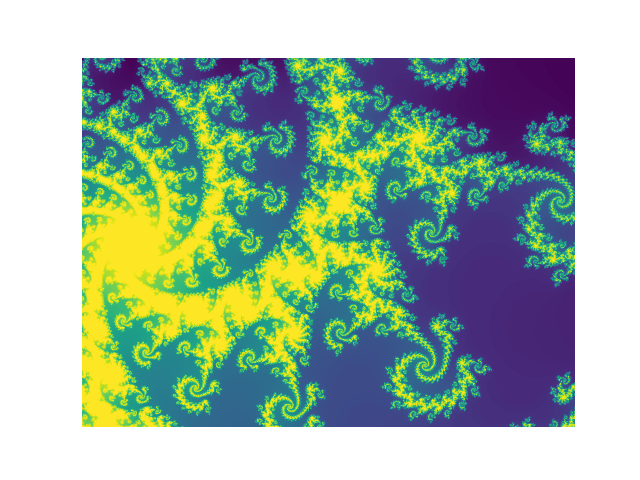
\includegraphics[height=5cm]{./result_zoom_2000.0.png}
\caption{Example generated figure of Mandelbrot Set with \emph{1024*768 resolution} and \emph{2000.0} times zoom in.}
\label{Mandelbrot Set Figure}
\end{center}
\end{figure}

There is another benefit of choosing the Mandelbrot Set. With the different combinations of image size, zoom level and colour depth, the cost of each task can be various. It avoids an ideal scenario where each task costs the same time and compute resource without randomness. This makes the experiments more meaningful and result in more possibilities.

\section{Instance Configuration}

I have launched three instances of AWS EC2\cite{ec2} and built a Zookeeper\cite{zookeeper} cluster with one leader and two followers. The tech stack is listed below:



\begin{enumerate}
\item \emph{Zookeeper} - to synchronize data and status across all nodes in the cluster. 
\item \emph{Python} - the scripts for starting and stopping all servers and clients.
\item \emph{Fabric} - to establish the SSH connection from a node.
\item \emph{Numpy} - the core library for computation and storage.
\item \emph{Matplotlib} - the library to plot the figure from the two-dimensional array.
\end{enumerate}



It is also easy to scale the number of instances up and down. A user is able to edit the config file in the repository and manually add or delete an instance from the cluster.


\section{Server Topology}

There are two types of servers in the cluster: master server and worker server. With the default setting, each instance will launch one master server and three worker servers. So, it gives 3 master servers and 9 worker servers running at the same time. But only one master is doing the actual work of task assignment. The other masters will join the election queue and become backups of the current master. 

\subsubsection{Master Server}

A master server is aiming for assigning tasks which created by a client to all free workers. It also has the job to listen to any status change for all workers and clients. So it ensures that  every client can be served and no blocked task in the task queue when a worker died.

\subsubsection{Worker Server}

A worker server is aiming for computing the task that is assigned by the master. It will write the result back to the corresponding client's task path. Each worker has its own identity and life cycle in the cluster. Therefore, there is no effect on other cluster components when a worker added or died.


\begin{figure}[htbp]
\begin{center}
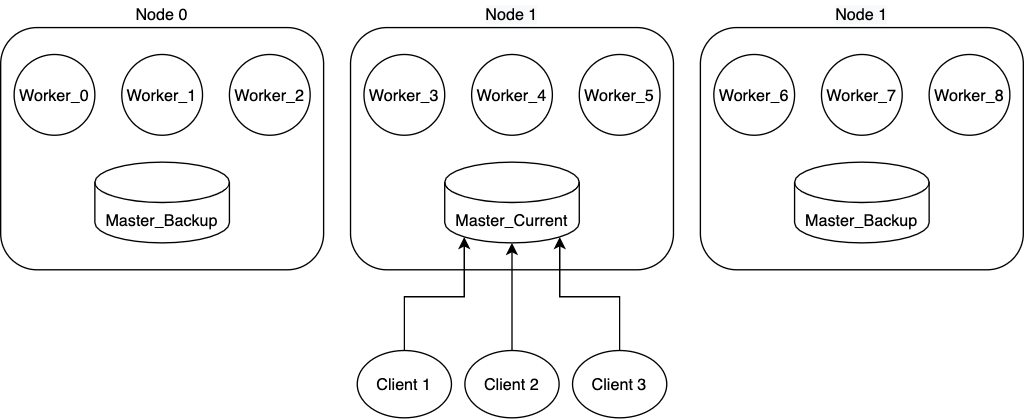
\includegraphics[height=4.8cm]{./ServerTopo.png}
\caption{Server Topology with 3 nodes running 1 master, 9 workers and 2 master backups.}
\label{Server Topology}
\end{center}
\end{figure}


\subsubsection{Election of Master}
Every time the system reboots or the current master dies, a ballot of election will takes place. One of the master candidates will become the new master. This election algorithm always picks the candidate with the smallest sequence id.



\subsubsection{Znode Design}
Znode is the core feature of Zookeeper used for synchronizing. The watching mechanism of Znode can help a component know the latest event taken place in the cluster. All types of Znode are listed:

\begin{enumerate}
\item \textbf{/master/\{master id\}} - the children of this path are all masters' id, a child node is ephemeral with master connection. All masters will watch this path. If the current master dies, all master backups will elect a new master.
\item \textbf{/workers/\{worker id\}} -  the children of this path are all workers' id, a child node is ephemeral with worker connection. All masters will watch this path.
\item \textbf{/status/\{worker id\}} - the children of this path are all workers' id with worker status inside, a child node is ephemeral with worker connection.
\item \textbf{/clients/\{client id\}} -  the children of this path are all clients' id, a child node is ephemeral with client connection. All masters will watch this path.
\item \textbf{/tasks/\{task id\}} - the children of this path are all tasks' id with task status, its client id and assigned worker id inside. Each task child node is ephemeral with its client connection.
\item \textbf{/params/\{task id\}} - the children of this path are all tasks' id with the parameters of task inside. Each parameter child node is ephemeral with its client connection.
\item \textbf{/results/\{client id\}/\{task id\}} -  the children of this path are all tasks' id with the compute result of each task inside. Each result node is persistent. All clients will watch this path.
\end{enumerate}

\section{Client Implementation}

The main job of a client is to divide the figure into multiple sub-tasks and send them to the task queue. Each task contains a slice of the final figure of the Mandelbrot Set. A user can input the number of slices in the client to tell the client how many sub-tasks to send. For instance, a user inputs value 6 means a client will slice the figure into 6 uniform pieces horizontally. A sub-task contains multiple parameters: start row index, end row index, resolution of the output and zoom level of the Mandelbrot Set. After sending a task out, the client will watch the \emph{/result} path until all tasks have a result write back.

An example of task generation is slicing 1024*768 figure into 3 pieces with 1 zoom level. The client will generate following sub-tasks finally:
\begin{verbatim}
/tasks/0_0000000395 b'client_id'
/params/0_0000000395 b'1024:768:1.0:0:256'
/tasks/1_0000000396 b'client_id'
/params/1_0000000396 b'1024:768:1.0:256:512'
/tasks/2_0000000397 b'client_id'
/params/2_0000000397 b'1024:768:1.0:512:768'
\end{verbatim}

Each parameter data indicates: \emph{height:width:zoom:start\_row:end\_row}. The master also watches the \emph{/tasks} path at the same time. Therefore, if there is a new task created, the task assignment procedure will be called.

\section{Scalability}
Scaling up or down the number of worker servers is easy by editing the variable in file \emph{start\_server.py}. 

\begin{verbatim}
#edit these lines to declare number of server
MASTER_NUM_ON_EACH_NODE = 1  
WORKER_NUM = 6   # deploy uniformly on all nodes

#terminal
> python start_server.py master
> python start_server.py worker
\end{verbatim}
This script will stop all servers and redeploy them. To manually add a new master or worker without stopping the existing servers, a user can use the following commands to run a server in foreground.

\begin{verbatim}
#terminal
> make master   # adding a new master
> make worker   # adding a new worker
\end{verbatim}

To test the scalability of the cloud application, the following experiment will scale up the number of worker servers. In this experiment, each worker will processes 1 task. As recorded in the following table, the number of workers is scaled up from 1 to 6. The client send a task with inputing 1024*768 resolution and 100.0 zoom level.

\begin{table}[htp]
\caption{TIme cost vs number of workers}
\begin{center}
\begin{tabular}{|c|c|}
\hline
Number of Workers & Time cost of task in seconds \\ \hline
1                 & 27.27s                       \\ \hline
2                 & 16.15s                       \\ \hline
3                 & 15.13s                       \\ \hline
4                 & 14.8s                        \\ \hline
5                 & 13.32s                       \\ \hline
6                 & 12.26s                       \\ \hline
\end{tabular}
\end{center}
\label{default}
\end{table}%

The table clearly shows the benefits of scaling up the worker servers. In the case of one worker, only one node is doing the computation. Two workers bring an obvious improvement on the speed. The time decreasing is less obvious with more workers. It brings more communication between master and worker to sync each task status, therefore, more time cost.

\section{Fault Tolerant}

The previous implementation section shows how the whole system is established. In this section, it introduces multiple experiments to test the fault-tolerant feature. There are different fault scenarios. I will label each case in a short form where \emph{M} represents \emph{Master}, \emph{W} represents \emph{Worker} and \emph{C} represents \emph{Client}. Three cases are introduced:

\begin{enumerate}
\item  \emph{2M:2W:1C} to \emph{1M:2W:1C} - test 1 master fails
\item  \emph{2M:2W:1C} to \emph{2M:1W:1C} - test 1 worker fails
\item  \emph{2M:2W:1C} to \emph{2M:0W:1C} - test all worker fails
\end{enumerate}

\subsection{Test 1 master fails - \emph{2M:2W:1C} to \emph{1M:2W:1C}}
This experiment will test the fail of the current master when a client is connecting to it.  An interrupt signal will stop the current master while it is in the halfway of a client task.
\begin{verbatim}
----------
python ./app/master.py   # master 1
...
My id is:  id_0000000034
Master is: /master/master_current/id_0000000034
I am master now
...
#Interrupt signal
----------
python ./app/master.py.  # master 2
...
My id is:  id_0000000035
Master is: /master/master_current/id_0000000034
I am master backup now
Master just died, new master election start...
Master is: /master/master_current/id_0000000035
I am master now
----------
\end{verbatim}

The result shows that the master can transfer to a new one when the old one is killed by an interrupt signal. In this case, all workers can get a task from master and clients can get the correct result in the end. So it tolerates the current master fault.

\subsection{Test 1 worker fails - \emph{2M:2W:1C} to \emph{2M:1W:1C}}

This experiment will test the fail of a worker when it is processing a client's task.  An interrupt signal will stop one of two workers.

\begin{verbatim}
----------
python ./client.py   # client 1
2 workers
1 masters
create: /results/client_3c161852-d05f-46db-8f84-790dd0d7623a
enter number of slices to deploy: 10
...
task progress: 1/10
task progress: 2/10
1 workers. # one of the worker dies
task progress: 3/10. # the task is still running
task progress: 4/10
...
----------
python ./app/master,oy.  # master
...
Worker died 1e2fe38f with status: 1_0000000429 
Task free: 1_0000000429.   # free the task from died worker
...
Try to distribute 1_0000000429 to worker: 9a928e11 
...
----------
\end{verbatim}

The output shows there is no effect when one of the workers dies. This is because the master will free the assigned task from the died worker and assign it to a new worker. Therefore, the application can tolerate this scenarios.

\subsection{Test all worker fails - \emph{2M:2W:1C} to \emph{2M:0W:1C}}
This experiment will test the fail of all workers when they are processing a client's task. All workers are stopped by an interrupt signal. Then I will launch a new worker to see if a client task can be recovered.

\begin{verbatim}
----------
python ./client.py   #client 1
2 workers
1 masters
create: /results/client_3c161852-d05f-46db-8f84-790dd0d7623a
enter number of slices to deploy: 10
...
task progress: 0/10
task progress: 1/10
0 workers.   # all worker fails, client stucks here
...
1 workers.   # relaunch a new worker, task is recovered
task progress: 2/10
2 workers
task progress: 3/10
...
----------
\end{verbatim}
The output shows a client will wait if all workers die and it can be recovered when at least one worker is relaunched.

All experiments have proved that this cloud application is resilient to various fault scenarios. With the larger scale of server deployments, the service will become more stable and highly available. There are four highlights in the design of the system to ensure its fault-tolerant feature:

\begin{enumerate}
\item Election -  to ensure there is always a master working.
\item Unblocked Task - a task will always free from a died worker.
\item Independent Client Status - each client has an ephemeral node to store its status.
\item Persistent Result -  all client result is stored persistently and can only be accessed by the master.
\end{enumerate}



\section{Conclusion}

This cloud application can compute the Mandelbrot Set in multiple embarrassingly parallelisable tasks. It is resilient to various fault scenarios and easy to scale up or down. It also supports numbers of clients to connect at the same time. At the end of the task, a beautiful figure of Mandelbrot Set will be generated. 

\begin{thebibliography}{4}

\bibitem{parallel}Wikipedia contributors, "Embarrassingly parallel," Wikipedia, The Free Encyclopedia, \url{https://en.wikipedia.org/w/index.php?title=Embarrassingly_parallel&oldid=988058646} (accessed December 4, 2020).

\bibitem{Mandelbrot}Wikipedia contributors, "Mandelbrot set," Wikipedia, The Free Encyclopedia, \url{https://en.wikipedia.org/w/index.php?title=Mandelbrot_set&oldid=991934444} (accessed December 4, 2020).

\bibitem{ec2}Wikipedia contributors, "Amazon Elastic Compute Cloud," Wikipedia, The Free Encyclopedia, \url{https://en.wikipedia.org/w/index.php?title=Amazon_Elastic_Compute_Cloud&oldid=991810523} (accessed December 6, 2020).

\bibitem{zookeeper}"Zookeeper" Apache ZooKeeper \url{https://zookeeper.apache.org/} (accessed December 6, 2020).


\end{thebibliography}

\section*{Appendix}

GitHub Repository: \url{https://github.com/ccdb-uob/CW20-20}

\end{document}
